\documentclass[10pt,a4paper,ngerman]{scrartcl}
\usepackage[utf8]{inputenc}
\usepackage[ngerman]{babel}
\usepackage[T1]{fontenc}
\usepackage{amsmath}
\usepackage{amsfonts}
\usepackage{amssymb}
\usepackage{makeidx}
\usepackage{graphicx}
\usepackage{epstopdf}
\usepackage[onehalfspacing]{setspace}
\usepackage{array}
\usepackage{upgreek}
\usepackage{float}
\usepackage{csquotes}
\usepackage{chemformula}
\usepackage{chemgreek}
\usepackage{chemmacros}
\chemsetup{modules=all}
\usepackage{tikz}
\usepackage{siunitx}
\sisetup{locale = DE,per-mode = symbol}
\usepackage{esvect}
\usepackage{geometry}
\usepackage{pdfpages}
\usepackage[font=small]{caption}
%\usepackage[version=4]{mhchem}
\usepackage[backend=biber, style=chem-angew]{biblatex}
\addbibresource{Raft.bib}
\usepackage{tabularx, booktabs, multirow}
\usepackage[pdfborder={0 0 0}]{hyperref}
\usepackage{scrlayer-scrpage}%Header für die KOMA-script -Klasse
%\usepackage{hyperref}
\usepackage{pgfplots}
\usepackage{textgreek}


\newcommand{\tildenu}{{\fontencoding{LGR}\selectfont\accperispomeni\textnu}}
\captionsetup{format=plain}
\chemsetup[phases]{pos=sub}
\chemsetup[redox]{pos=top}
\chemsetup[redox]{align=center}
%\chemsetup[redox]{explicit-sign=true}
%\chemsetup[redox]{roman=false}
\newcommand{\celsius}{^{\circ}\mathrm{C}}
\parindent0pt
\sloppy
\DeclareChemPhase{\s}{s}
\DeclareChemPhase{\l}{l}
\DeclareChemPhase{\g}{g}
\renewcaptionname{ngerman}{\figurename}{Abb.}
\renewcaptionname{ngerman}{\tablename}{Tab.}
\geometry{bottom=100pt} \geometry{top=80pt}
\newcommand{\m}{\mathrm{m}}
\newcommand{\K}{\mathrm{K}}
\newcommand{\J}{\mathrm{J}}
\newcommand{\gr}{\mathrm{g}}
\newcommand{\kg}{\mathrm{kg}}
\newcommand{\mol}{\mathrm{mol}}
\newcommand{\Pa}{\mathrm{Pa}}
\newcommand{\ad}{\mathrm{ad}}
\newcommand{\de}{\mathrm{de}}
\newcommand{\gmol}{\mathrm{\frac{g}{mol}}}
\newcommand{\JKmol}{\mathrm{\frac{J}{K \cdot mol}}}
\newcommand{\kgmss}{\mathrm{\frac{kg}{m \cdot s^2}}}
\newcommand{\loge}{\mathrm{ln}}


\begin{document}
\begin{titlepage}
	\vspace*{2,5cm}
	\begin{center}
		\begin{LARGE}
			\textbf{Polymer Chemie}\\
			\textbf{RAFT}\\
		\end{LARGE}
		\vspace{1cm}
		\textbf{Universität Stuttgart}\\
		\vspace*{1,5cm}
		\begin{tabular}{lp{7,5cm}l}
			Author 1:     &Laurens Viehoff\\
            Author 2:     &Felix Roth\\   
			E-Mail 1:      &st183688@stud.uni-stuttgart.de\\
            E-Mail 2:      &st188157@stud.uni-stuttgart.de  \\
			Student-ID 1: & 3676761   \\ 
            Student-ID 2: & 3711192 \\ \\
			Assistentin:  & Alina Tengler \\ \\ 
		\end{tabular}
	\end{center}

    
\end{titlepage}
\thispagestyle{empty}
\renewcommand{\thepage}{\arabic{page}}
\newpage
\tableofcontents
\setcounter{page}{1}
\renewcommand{\thepage}{\arabic{page}}
\newpage

\section{Theorie}

	\subsection{Kontrollierte radikalische Polymerisation}

		Die freie radikalische Polymerisation ist eine leichte und breit anwendbare Polymerisation, welche allerdings nur bedingt lange Polymere und eine breite 
		Molmassenverteilung aufweist. Daher wurden kontrollierte radikalische Polymerisationen entwickelt, bei welchen längere Ketten und definiertere Molmassenverteilungen 
		möglich sind. Das Problem an der radikalische Polymerisation sind die Abbruchreaktion, welche sehr häufig und schnell auftreten. Um dieses Problem zu umgehen, 
		kann beispielsweise die Radikalkonzentration herabgesenkt werden, da somit die Häufigkeit an Terminierungsreaktion quadratisch abfällt. Um dies zu bewirken wird die 
		aktive Radikalspezies in ein Gleichgewicht eingebunden, bei welchem das Radikal wahrscheinlicher im \textquotedblleft schlafenden\textquotedblright $\,$ Zustand vorliegt. Dies kann beispielsweise mit 
		stabilen Radikalen, wie Nitroxide oder Übergangsmetalle geschehen. Die Methoden dazu wären einmal die Nitroxid-vermittelte-Polymerisation (NMP) und die 
		$Atom$ $Transfer$ $Radical$ $Polymerization$ (ATRP). Eine weitere Methode der kontrollierten radikalischen Polymerisation ist die 
		$Reversible$ $Addition/Fragmentation$ $Chain$ $Transfer$ $Polymerization$ (RAFT). \cite{polyskript}

		\subsubsection{RAFT}

			Bei der RAFT-Polymerisation wird die Radikalkonzentration nicht herabgesenkt, sondern die Kettenlänge kontrolliert. Das geschieht dadurch, dass bei 
			desaktivierung einer Kette, eine andere Kette aktiviert wird und Polymerisieren kann. Die desaktivierten Ketten werden dann durch eine aktivierte 
			Polymerkette aktiviert, wodurch diese Polymerisieren kann. Das ganze führt dann dazu, dass die Ketten ein ähnliches Molekulargewicht besitzen.
			Die Addition einer aktiven Kette und fragmentierung einer desaktivierten Kette erfolgt über eine Thiocarbonylthiogruppe wie sie in Abbildung \ref{RAFTGruppe}
			gezeigt ist. 

			\begin{figure}[H]
				\centering
				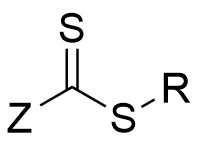
\includegraphics[scale = 0.35]{Bilder/RAFT-Gruppe.png}
				\caption{Allgemeiner Aufbau einer Thiocarbonylthiogruppe.}
				\label{RAFTGruppe}
			\end{figure}

			Dabei ist wichtig, dass die C=S-Bindung gegenüber Radikalen eine gewisse Reaktivität aufweist. Das wird über den Substituenten $Z$ erreicht, welcher das 
			Radikal-Intermediat stabilisiert. Des weiteren muss die R-S-Bindung homolytisch Spaltbar sein und $R$ muss ein Radikal sein, welches ebenfalls eine Polymerisierung 
			initiieren können. Für diese Anforderungen gibt es verschiedene Substituenten, die ebenfalls in vier Untergruppen eingeteilt werden können. Die möglichen 
			RAFT-Reagenzien sind in Tabelle \ref{RAFTReagenzien} aufgeführt.

			\begin{figure}[H]
				\centering
				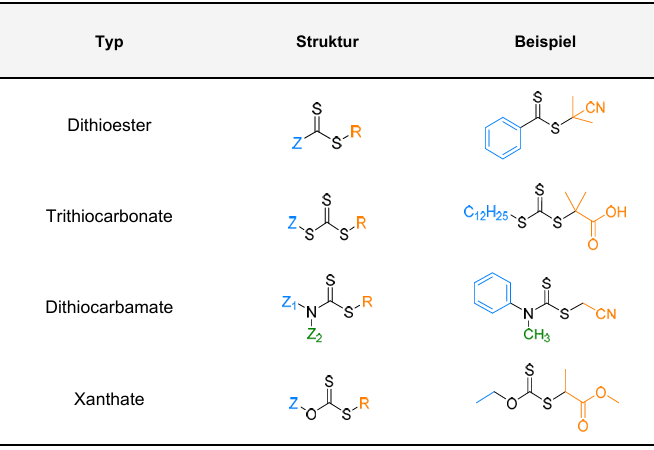
\includegraphics[scale = 0.8]{Bilder/RaftGruppentabular.png}
				\caption{RAFT-Ragenzien mit Struktur und einem Beispiel. \cite{polyskript}}
				\label{RAFTReagenzien}
			\end{figure}

			Diese RAFT-Ragenzien sind für unterschiedliche Monomere unterschiedlich gut geeignet und sind somit Monomer spezifisch. So gibt es zum Beispiel stark aktivierte
			Monomere (MAMs) und weniger stark aktivierte Monomere (LAMs). Bei MAMs werden die entstehenden Radikale durch Substituenten stabilisiert. Dafür sind 
			beispielsweise konjugierte Doppelbindungen, konjugierte Aromaten oder Kohlenstoffketten substituiert. Da MAMs ihre Radikale gut stabilisieren, müssen die 
			RAFT-Ragenzien ebenfalls das Radikal stabilisieren, wobei hierfür Dithioester oder Trithiocarbonate am besten geeignet sind. LAMs hingegen stabilisieren das 
			entstehende Radikal nicht sonderlich gut und benötigen somit RAFT-Reagenzien, die das Radikal weniger gut stabilisieren. Die Polymerisierung wird dann über 
			Dithiocarbamate oder Xanthanate gesteuert. \\
			Für ein besseres Verständnis ist der Reaktionsmechanismus der RAFT-Polymerisation in Abbildung \ref{RAFTMechanismus} aufgeführt.

			\begin{figure}[H]
				\centering
				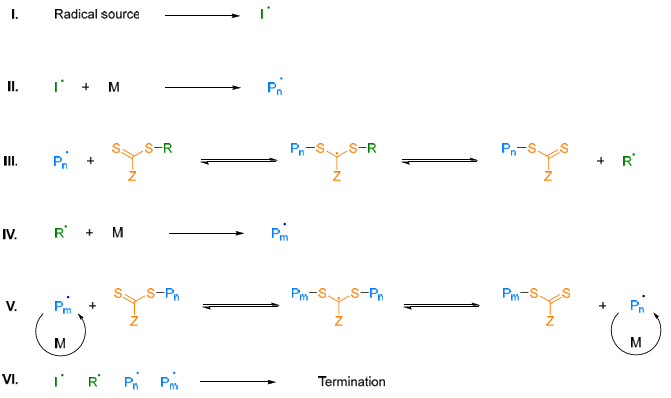
\includegraphics[scale = 0.8]{Bilder/RAFT-Mechanismus.png}
				\caption{Mechanismus der RAFT-Polymerisation unter Verwendung eines Dithioesters. \cite{polyskript}}
				\label{RAFTMechanismus}
			\end{figure}

			Zu Beginn wird ein Radikal aus einer Radikalquelle freigesetzt (I), welches mit Monomer polymerisiert (II) und zu jeder Zeit an die RAFT-Ragenz koordinieren 
			kann (III). Durch die Addition eines Radikals entsteht das Zwischenprodukt, welches zum einen durch $Z$ stabilisiert wird und zum anderen das $R$-Radikal 
			freisetzen kann. Dieses Radikal kann erneut Polymerisieren (IV) und anschließend ebenso an das RAFT-Reagenz addieren, wodurch es die andere Kette freisetzt (V). 
			Zum Schluss können Radikale, welche nicht koordiniert sind jeder Zeit rekombinieren und somit die Kette terminieren (VI). \\
			Die Gleichgewichte (III) und (V) sind dabei essenziell, da darüber die Kettenlängen kontrolliert werden und so ein optimaler PDI und optimale Kettenlänge erziehlt 
			werden kann. Des weiteren wird bei diesen Gleichgewichten noch deutig, warum die stabilisierung durch $Z$ so wichtig ist. Wird dieses Radikal beispielsweise
			durch ein Phenyl-Substituenten stabilisiert, während das Monomer das Radikal nicht sonderlich gut stabilisiert, wird das Gleichgewicht in Richtung der 
			Zwischenstufe gedrückt und die Reaktion (IV) verläuft nicht sehr oft. Bei umgekehrter stabilisierung würde das Gleichgewicht in Richtung der aktiven Radikale 
			gedrückt werden, wodurch die Reaktion einer freien radikalischen Reaktion ähneln würde.\\
			Um nun eine optimale RAFT-Reaktion zu bedingen, werden die Reagenzien häufig im Verhältnis [I]/[RAFT]/[M] = [1]/[4-10]/[2000-5000] vorgelegt. Des weiteren kann 
			dann das Molekulargewicht der Reaktion über die Gleichung \eqref{Molekulargewicht} berechnet werden.

			\begin{equation}
				M_\text{n,Calc} = \bigl(X \cdot \frac{[\text{M}]_0}{[\text{RAFT}]_0} \cdot m\text{M}\bigr) + m\text{RAFT}
				\label{Molekulargewicht}
			\end{equation}

			$M_\text{n,Calc}$ ist dabei das berechnete Molekulargewicht, $X$ der Monomerumsatz, $m\text{M}$ und $m\text{RAFT}$ beschreiben das Molekulargewicht des Monomers
			und der RAFT-Reagenz und $[\text{M}]_0$ und $[\text{RAFT}]_0$ beziehen sich auf die Anfangskonzentration von Monomer und RAFT-Reagenz. \cite{polyskript}



\section{Auswertung}



\section{Durchführung}



\section{Fragen}
\printbibliography

\end{document}